\documentclass{beamer}

\usetheme[progressbar=frametitle]{metropolis}
\usepackage{appendixnumberbeamer}
\usepackage{booktabs}
\usepackage{amsmath}
\usepackage{amssymb}
\usepackage{tcolorbox}
\usepackage{tikz}

\definecolor{metropolisblue}{RGB}{39, 59, 94}



% Begin document
\begin{document}

% Title page
\title{Sampling Methods}
\author{Nipun Batra}
\date{\today}
\institute{IIT Gandhinagar}
\maketitle

\begin{frame}{Topics}
    %TOC with enumerated items
    \setbeamertemplate{section in toc}[sections numbered]
    \tableofcontents[hideallsubsections]

\end{frame}

\begin{section}{Monte Carlo Simulation}

    \begin{frame}{The idea behind MC Simulation}
        \begin{itemize}
            \item We often want to compute expected value of some function of a random variable, which turns into the integral, 
            $$\mathbb{E} \left[ f (x) \right] = \int f(x) p(x) dx$$
            where $x \in \mathbb{R}^n, f: \mathbb{R}^n \rightarrow \mathbb{R}^m$ and $p(x)$ is the target distribution.
            \item In low dimensions, we can use numerical integration techniques to compute the above integral. However, in high dimensions, this is not feasible.
            \item Alternative approach is to draw  multiple random samples, $x_i \sim p(x)$ and compute
            $$\mathbb{E} \left[ f (x) \right] \approx \frac{1}{N} \sum_{i=1}^{N} f(x_i)$$
        \end{itemize}
    \end{frame}

    \begin{frame}{General Form}

        The general form of Monte Carlo methods is:
        The expectation of a function $f(x)$ with respect to a distribution $p(x)$ is given by:
        \begin{equation}
            % Expectation of f(x) with respect to p(x)
            \mathbb{E}_{x \sim p(x)}[f(x)] = \int f(x) p(x) dx
        \end{equation}
        
        Using Monte Carlo methods, we can estimate the above expectation by sampling $x_i$ from $p(x)$ and computing the average of $f(x_i)$.
        \begin{equation}
            % Monte Carlo estimate of expectation of f(x) with respect to p(x)
            \mathbb{E}_{x \sim p(x)}[f(x)] \approx \frac{1}{N} \sum_{i=1}^{N} f(x_i)
        \end{equation}
        where $x_i \sim p(x)$.

    \end{frame}

    % \begin{frame}{ }
    %     It is often difficult to compute the intergral $\int f(x) p(x) dx$ as it is expensive or intractable.
        
    %     Using Monte Carlo methods, we can estimate by sampling $x_i$ from $p(x)$ and computing the average of $f(x_i)$.
    %     \begin{equation}
    %         % Monte Carlo estimate of expectation of f(x) with respect to p(x)
    %         \mathbb{E}_{x \sim p(x)}[f(x)] \approx \frac{1}{N} \sum_{i=1}^{N} f(x_i)
    %     \end{equation}
    %     where $x_i \sim p(x)$.

    %     \begin{equation}
    %         % Expectation of f(x) with respect to p(x)
    %         \mathbb{E}_{x \sim p(x)}[f(x)] = \int f(x) p(x) dx
    %     \end{equation}
    %     Thus we can approximate the induced distribution, $p(x)$ sampling $x_i$ from $p(x)$ and computing the average of $f(x_i)$.
    % \end{frame}

    \begin{frame}{Unbiased Estimator?}
        Is Monte Carlo Sampling a biased or unbiased estimator?

        We know:
        \begin{equation}
            % Expectation of f(x) with respect to p(x)
            \mathbb{E}_{x \sim p(x)}[f(x)] = \int f(x) p(x) dx = \phi
        \end{equation}
        Let $x_i\in 1, \ldots, N$ be i.i.d samples:
        \begin{align*}
            \hat{\phi} &= \frac{1}{N} \sum_{i=1}^{N} f(x_i) \\
            \mathbb{E}(\hat{\phi}) &= \int \frac{1}{N} \sum_{i=1}^{N} f(x_i)p(x_i)dx = \frac{1}{N}\sum_{i=1}^{N} \int f(x_i)p(x_i)dx \\
            &= \frac{1}{N}\sum_{i=1}^N\mathbb{E}(f(x_i)) = \phi
        \end{align*}
        Thus, it is an unbiased estimator!
    \end{frame}

    \begin{frame}[fragile]{Estimating Pi using Monte Carlo (Part 1)}
        We can estimate the value of pi using Monte Carlo methods by considering a unit square with a quarter circle inscribed within it.
        
        \begin{itemize}
            \item Let $p(x)$ be defined over the unit square using the uniform distribution in two dimensions, i.e., $p(x) = U(x) = 1$ for $x \in [0, 1]^2$.
            \item Let $f(x)$ be the indicator function defined as follows:
                \[
                f(x) = \begin{cases}
                            \text{\textcolor{green}{Green}} (1), & \text{if } x \text{ falls inside the quarter circle}, \\
                            \text{\textcolor{red}{Red}} (0), & \text{otherwise}.
                       \end{cases}
                \]
        \end{itemize}
    \end{frame}

    \begin{frame}[fragile]{Estimating Pi using Monte Carlo (Part 1)}

        \begin{itemize}
        \item Or, we can write $f(x)$ to be the following:
            \[
            f(x) = \begin{cases}
                        1, & \text{if } x_1^2 + x_2^2 \leq 1, \\
                        0, & \text{otherwise}.
                   \end{cases}
            \]
        \item Or, using the indicator function, we can write $f(x)$ to be the following:
            \[
            f(x) = \mathbb{I}(x_1^2 + x_2^2 \leq 1)
            \]
        \end{itemize}
        
        \begin{center}
            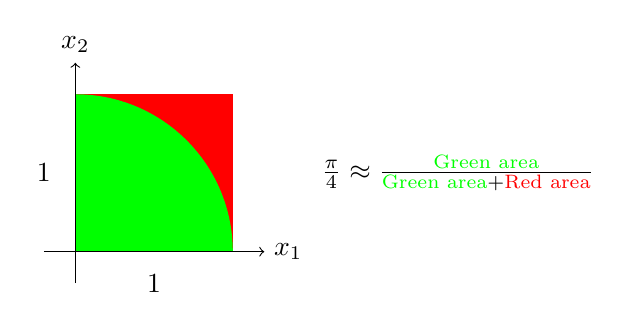
\begin{tikzpicture}[scale=2]
                % Unit Square
                \fill[red] (0,0) rectangle (1,1);
                
                % Quarter Circle
                \fill[green] (0,0) -- (0,1) arc (90:0:1) -- cycle;
                
                % Coordinate Axes
                \draw[->] (-0.2,0) -- (1.2,0) node[right] {$x_1$};
                \draw[->] (0,-0.2) -- (0,1.2) node[above] {$x_2$};
                
                % Labels
                \node at (0.5, -0.2) {1};
                \node at (-0.2, 0.5) {1};
                \node[right] at (1.5, 0.5) {$\frac{\pi}{4} \approx \frac{\text{\textcolor{green}{Green area}}}{\text{\textcolor{green}{Green area}} + \text{\textcolor{red}{Red area}}}$};
        
            \end{tikzpicture}
        \end{center}
    \end{frame}

    \begin{frame}
        \begin{figure}
                \centering
                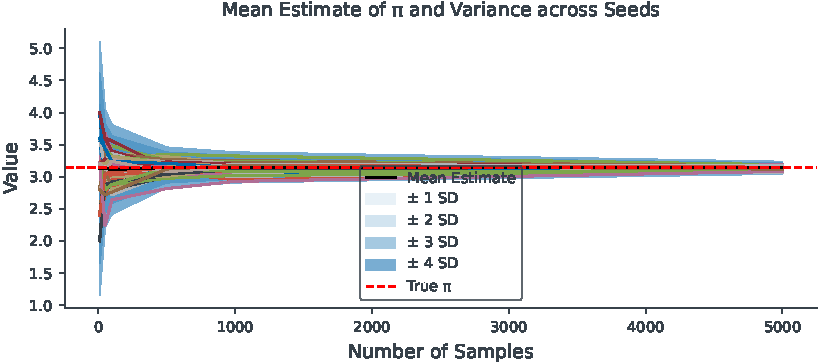
\includegraphics[scale = 0.8]{../figures/prediction_var_mc_pi.pdf}
            \end{figure}
    \end{frame}

    \begin{frame}{Estimating a function using Monte Carlo}
        Let $x\in \mathcal{U}(-1,1)$ and $y = f(x) = x^2$.
        \begin{figure}
            \centering
        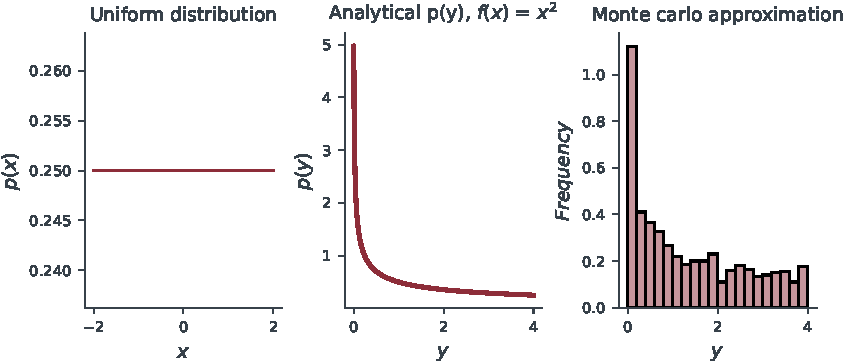
\includegraphics[scale=0.75]{../figures/mc_sampling_ex.pdf}
            \end{figure}    
    \end{frame}

    \begin{frame}{Sampling converges slowly}
        The expected square error of the Monte Carlo estimate is given by:
        $$
        \mathbb{E} \left( \hat{\phi} - \mathbb{E} (\hat{\phi}) \right)^2 = \mathbb{E} \left[ \frac{1}{N} \sum_{i=1}^{N} (f(x_i) - \phi) \right]^2 
        $$
        $$
        = \frac{1}{N^2} \sum_{i=1}^{N} \sum_{j=1}^{N} \mathbb{E} (f(x_i) f(x_j)) - \phi \mathbb{E} (f(x_i)) - \mathbb{E} (f(x_j)) \phi + \phi^2
        $$
        $$
        = \frac{1}{N^2} \sum_{i=1}^{N} \left( \left( \sum_{i \neq j}^{} \phi^2 - 2 \phi^2 + \phi^2 \right) + \mathbb{E} (f^2) - \phi^2 \right) = \frac{1}{N} \mathbb{V} (f)
        $$
        $$
        \therefore \mathbb{E} \left( \hat{\phi} - \mathbb{E} (\hat{\phi}) \right)^2 = \mathcal{O} (N^{-1})
        $$
        Thus, the expected error drops as $\mathcal{O} (N^{-\frac{1}{2}})$.
    \end{frame}

    \begin{frame}{Pop Quiz}
        How many samples ($N$) do we need to reach single-precision (i.e., $\sim 10^{-7}$)?
    \end{frame}

    \begin{frame}{Is sampling easy?}
        Many reasons contribute to sampling not always being easy in higher dimensions. For example,
        \begin{itemize}
            \item need a global description of the entire function
            \item need to know probability densities everywhere
            \item need to know regions of high density
        \end{itemize}
    \end{frame}

    \begin{frame}{Estimating prior predictive distribution}
        \begin{itemize}
            \item Let $p(\theta)$ be the prior distribution of parameter $\theta \in \mathbb{R}^2$. Say, for example, $p(\theta_i) = \mathcal{N}(0, 1) \forall i$.
            \item Let $p(y |\theta, x)$ be the likelihood function. Say, for example, $p(y|\theta, x) = \mathcal{N}(\theta_0 + \theta_1 x, 1)$.
            \item Then, the prior predictive distribution is given by:
        \end{itemize}

            \begin{equation}
                p(y|x) = \int p(y|\theta, x) p(\theta) d\theta 
            \end{equation}

            \begin{equation}
                p(y|x) \approx \frac{1}{N} \sum_{i=1}^{N} p(y|\theta_i, x)
            \end{equation}
            where $\theta_i \sim p(\theta)$.
    \end{frame}

    \begin{frame}{Estimating posterior predictive distribution}
        Extending for posterior predictive distribution, we have:

        \begin{equation}
            p(y|x, D) = \int p(y|\theta, x) p(\theta|D) d\theta 
        \end{equation}

        \begin{equation}
            p(y|x, D) \approx \frac{1}{N} \sum_{i=1}^{N} p(y|\theta_i, x)
        \end{equation}
        
    \end{frame}

\end{section}

\begin{section}{Rejection Sampling}
    \begin{frame}{Rejection Sampling}
        \begin{itemize}
            \item Let $p(x)$ be the target distribution from which we want to sample.
            \item Let $q(x)$ be a proposal distribution from which we can sample.
            \item Let $M$ be a constant such that $M \geq \frac{p(x)}{q(x)} \forall x$.
            \item Then, we can sample from $p(x)$ by sampling from $q(x)$ and accepting the sample with probability $\frac{p(x)}{M q(x)}$.
        \end{itemize}
        
    \end{frame}

   \begin{frame}{Rejection Sampling}
    \begin{figure}
        \centering
        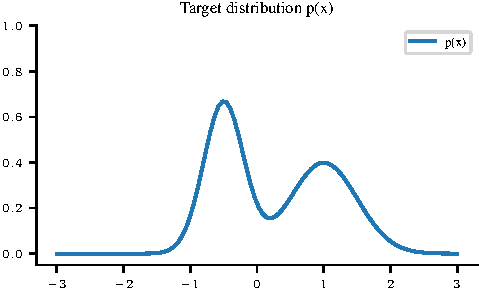
\includegraphics[scale = 0.75]{../figures/sampling/rejection-sampling--1.0-False-False-False-False-False-False-False-False.pdf}
    \end{figure}
    
   \end{frame}

    \begin{frame}{Rejection Sampling}
        \begin{figure}
            \centering
            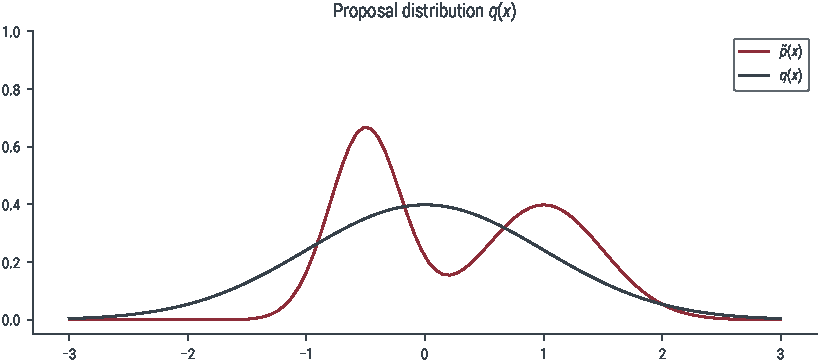
\includegraphics[scale = 0.75]{../figures/sampling/rejection-sampling--1.0-True-False-False-False-False-False-False-False.pdf}
        \end{figure}
    \end{frame}

    \begin{frame}{Rejection Sampling}
        \begin{figure}
            \centering
            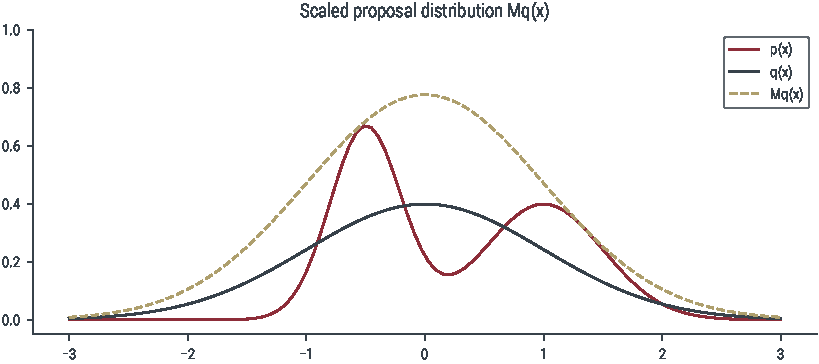
\includegraphics[scale = 0.75]{../figures/sampling/rejection-sampling--1.0-True-True-False-False-False-False-False-False.pdf}
        \end{figure}
    \end{frame}

    \begin{frame}{Rejection Sampling}
        \begin{figure}
            \centering
            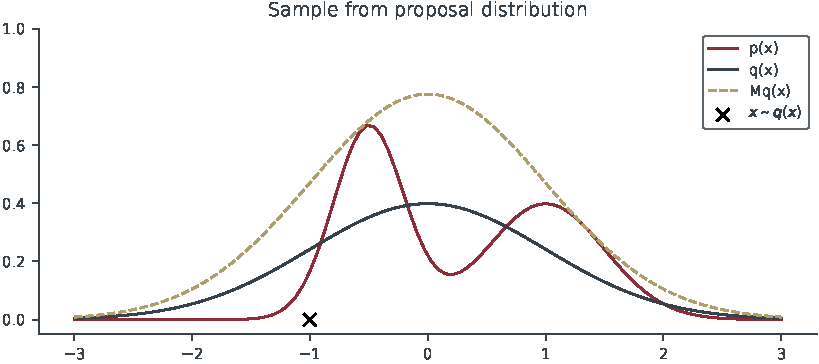
\includegraphics[scale = 0.75]{../figures/sampling/rejection-sampling--1.0-True-True-True-False-False-False-False-False.pdf}
        \end{figure}
    \end{frame}

    \begin{frame}{Rejection Sampling}
        \begin{figure}
            \centering
            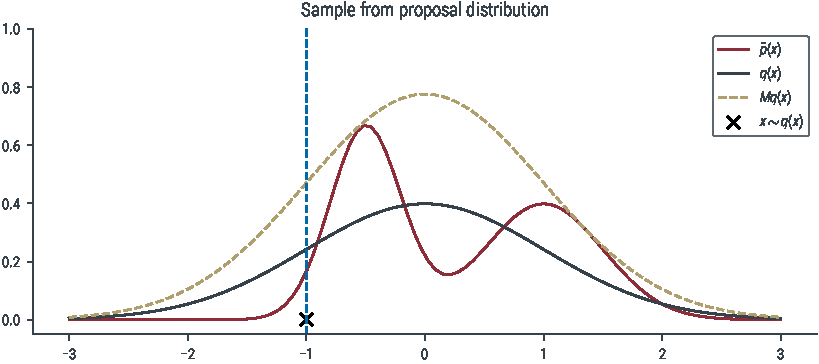
\includegraphics[scale = 0.75]{../figures/sampling/rejection-sampling--1.0-True-True-True-True-False-False-False-False.pdf}
        \end{figure}
    \end{frame}

    \begin{frame}{Rejection Sampling}
        \begin{figure}
            \centering
            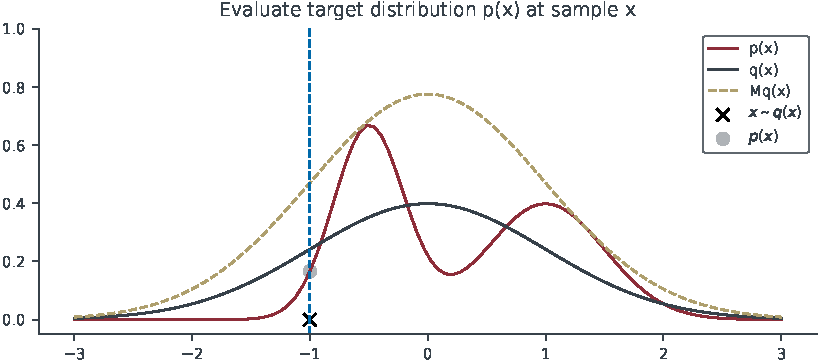
\includegraphics[scale = 0.75]{../figures/sampling/rejection-sampling--1.0-True-True-True-True-True-False-False-False.pdf}
        \end{figure}
    \end{frame}

    \begin{frame}{Rejection Sampling}
        \begin{figure}
            \centering
            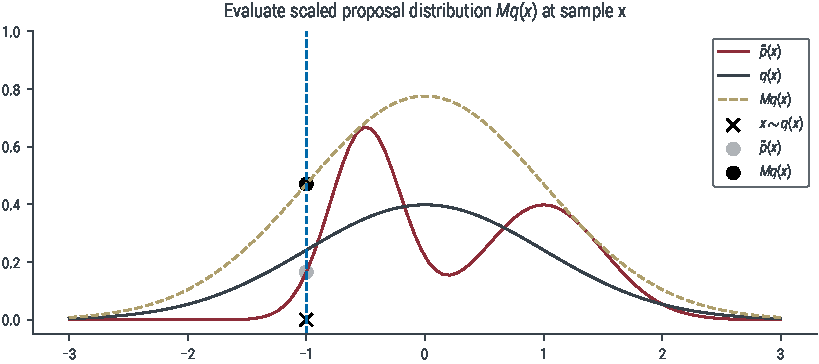
\includegraphics[scale = 0.75]{../figures/sampling/rejection-sampling--1.0-True-True-True-True-True-True-False-False.pdf}
        \end{figure}
    \end{frame}

    \begin{frame}{Rejection Sampling}
        \begin{figure}
            \centering
            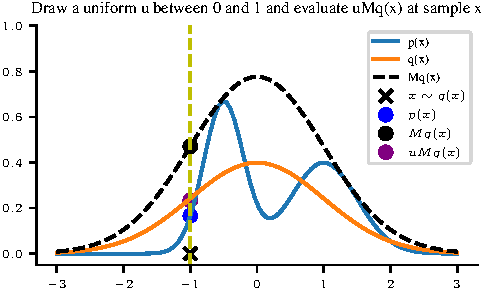
\includegraphics[scale = 0.75]{../figures/sampling/rejection-sampling--1.0-True-True-True-True-True-True-True-False.pdf}
        \end{figure}
    \end{frame}

    \begin{frame}{Rejection Sampling}
        \begin{figure}
            \centering
            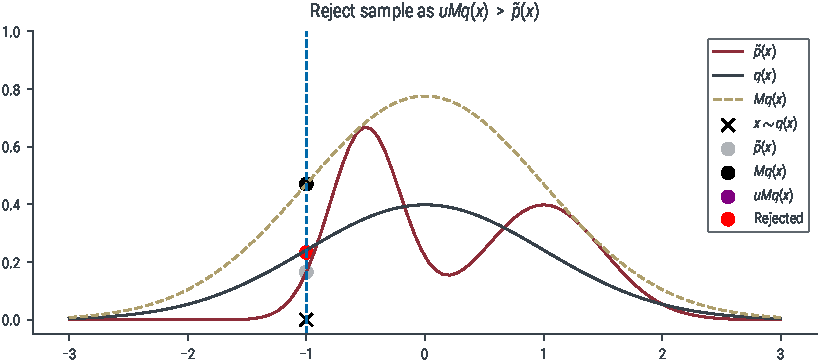
\includegraphics[scale = 0.75]{../figures/sampling/rejection-sampling--1.0-True-True-True-True-True-True-True-True.pdf}
        \end{figure}
    \end{frame}

    \begin{frame}{Proof of Rejection Sampling}
        \begin{tcolorbox}[colback=metropolisblue!5,colframe=metropolisblue,title={Acceptance Probability $\alpha(x)$}]
            \begin{equation}
              \alpha(x) = \frac{p(x)}{M q(x)}
            \end{equation}
        \end{tcolorbox}
       
        \begin{tcolorbox}[colback=metropolisblue!5,colframe=metropolisblue,title={Bayes Rule for Acceptance}]
            \begin{equation}
                P(Sample|Accept) = \frac{P(Accept|Sample) P(Sample)}{P(Accept)}
            \end{equation}
        \end{tcolorbox}

        \begin{tcolorbox}[colback=metropolisblue!5,colframe=metropolisblue,title={P(Sample)}]
            We draw samples from $q(x)$, so $P(Sample) = q(x)$.
        \end{tcolorbox}
    \end{frame}

    \begin{frame}{Proof of Rejection Sampling}

        Further, $P(Accept|Sample) = \alpha(x) = \dfrac{p(x)}{M q(x)}$.

        Finally, $P(Accept) = \int P(Accept|Sample) P(Sample) dSample = \int \alpha(x) q(x) dx = \dfrac{1}{M} \int p(x) dx = \dfrac{1}{M}$.
        \begin{tcolorbox}[colback=metropolisblue!5,colframe=metropolisblue,title={P(Accept)}]
            \begin{equation}
                P(Accept) = \frac{1}{M}
            \end{equation}
        \end{tcolorbox}
        

        Thus, $P(Sample|Accept) = \dfrac{p(x)}{M q(x)} \times \dfrac{q(x)}{1/M} = p(x)$.

        Thus, we have shown that the samples we accept are distributed according to $p(x)$.
        
    \end{frame}

    \begin{frame}{Rejection Sampling Completed Example}
        Note: Figures not on github.
    \end{frame}

    % \begin{frame}{Rejection Sampling Completed Example}
    %     \begin{figure}
    %         \centering
    %         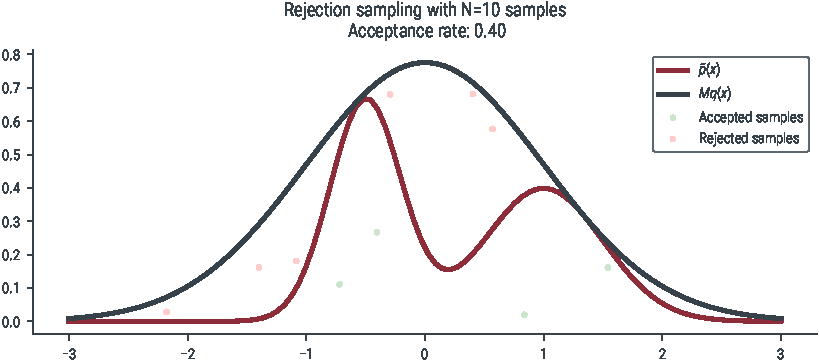
\includegraphics[scale = 0.75]{../figures/sampling/rejection-sampling-N10-False.pdf}
    %     \end{figure}
        
    % \end{frame}

    % \begin{frame}{Rejection Sampling Completed Example}
    %     \begin{figure}
    %         \centering
    %         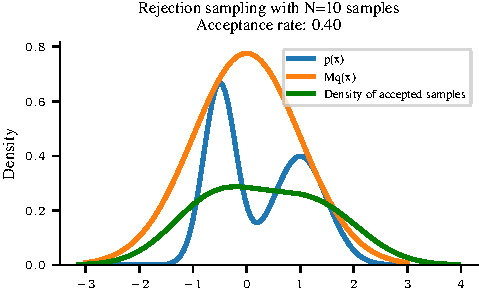
\includegraphics[scale = 0.75]{../figures/sampling/rejection-sampling-N10-True.pdf}
    %     \end{figure}
        
    % \end{frame}

    % \begin{frame}{Rejection Sampling Completed Example}
    %     \begin{figure}
    %         \centering
    %         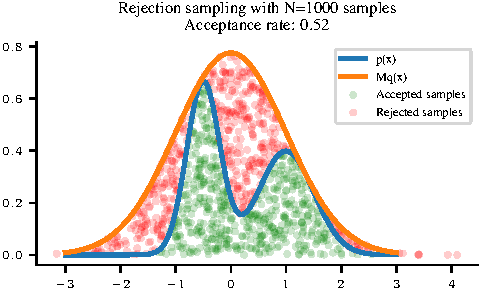
\includegraphics[scale = 0.75]{../figures/sampling/rejection-sampling-N1000-False.pdf}
    %     \end{figure}
    % \end{frame}

    % \begin{frame}{Rejection Sampling Completed Example}
    %     \begin{figure}
    %         \centering
    %         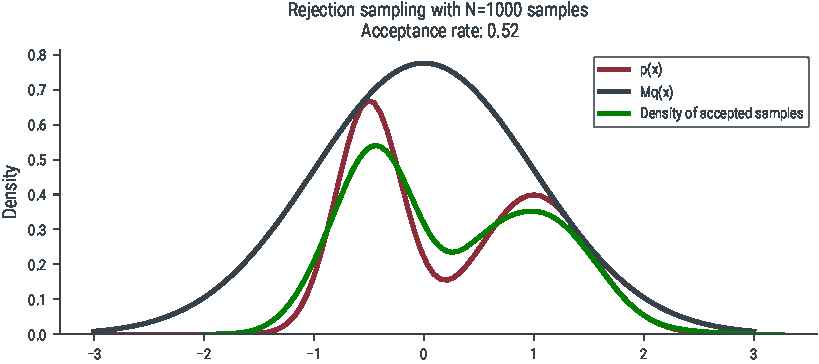
\includegraphics[scale = 0.75]{../figures/sampling/rejection-sampling-N1000-True.pdf}
    %     \end{figure}
    % \end{frame}

    % \begin{frame}{Rejection Sampling Completed Example}
    %     \begin{figure}
    %         \centering
    %         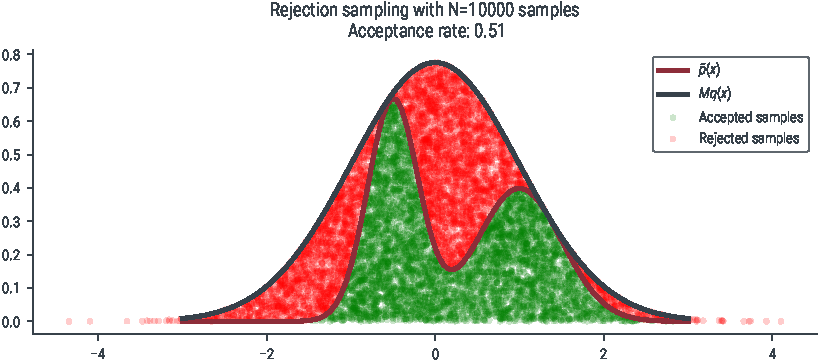
\includegraphics[scale = 0.75]{../figures/sampling/rejection-sampling-N10000-False.pdf}
    %     \end{figure}
    % \end{frame}

    % \begin{frame}{Rejection Sampling Completed Example}
    %     \begin{figure}
    %         \centering
    %         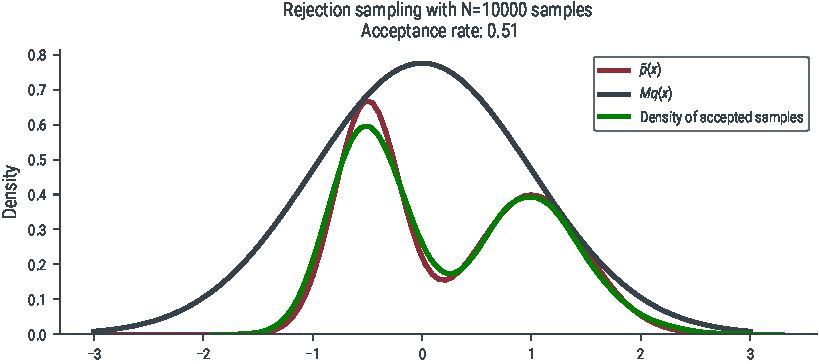
\includegraphics[scale = 0.75]{../figures/sampling/rejection-sampling-N10000-True.pdf}
    %     \end{figure}
    % \end{frame} 

    \begin{frame}{Challenges with Rejection Sampling}
        \begin{itemize}
            \item Rejection sampling is inefficient when the target distribution is very different from the proposal distribution.
            \item In this case, we will reject a lot of samples.
            \item This is a problem when sampling from high-dimensional distributions.
            \item Acceptance probability $\alpha(x)$ is very low.
        \end{itemize}
    \end{frame}

\end{section}

\begin{section}{Inverse CDF}
    \begin{frame}{General Form}
        Inverse Cumulative Distribution Function (Inverse CDF) sampling is a technique used to generate random numbers from a given probability distribution.

        Particularly useful when sampling from distributions lacking a straightforward analytical method for direct sampling. 
    \end{frame}

    \begin{frame}
        A method of sampling from the distribution is sampling $u\in \mathcal{U}(0,1)$ and find $x = F_X^{-1}(u)$. The cumulative probability distribution (cdf) of $X$ is:
        \begin{equation}
            F_X(x) = \mathbb{P}(X<=x) = \int_{-\infty}^{\infty} \pi(u)I(u<=x)du = \int_{-\infty}^{\infty}\pi(u)du 
        \end{equation}
        Thus, Sample $u\in \mathcal{U}(0,1)$ and set $Y=F_{\pi}^{-1}(u)$. 
    \end{frame}

    \begin{frame}{Proof}
        We need to prove that the algorithm mentioned above produces samples from $\pi$. We calculate the cdf of $X$ produced by the algorithm above. For any $y\in X$ we have:
        \begin{align*}
            \mathbb{P}(Y<=y) &= \mathbb{P}(Y=F_X^{-1}(u)<=y) \\
            &= \mathbb{P}(u<=F_X(y)) \\
            &= \int_0^1 I(u<=F_X(y)).1du = \int_0^{F_X(y)}du = F_X(y)
        \end{align*}
        This shows that the cdf of $Y$ produced by the algorithm is the same as cdf of $X\sim \pi$.
    \end{frame}

    \begin{frame}{Example of Normal distribution}
        Number of samples = 25:
        \begin{figure}
                \centering
                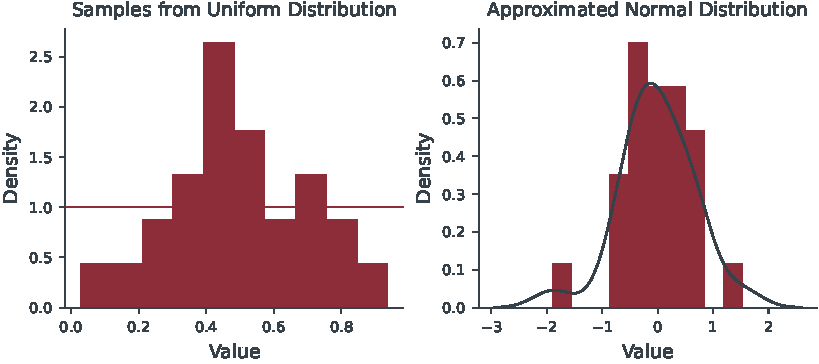
\includegraphics[scale=0.8]{../figures/inverse_cdf_normal1.pdf}
        \end{figure}
    \end{frame}
    \begin{frame}
        Number of samples = 100:
        \begin{figure}
                \centering
                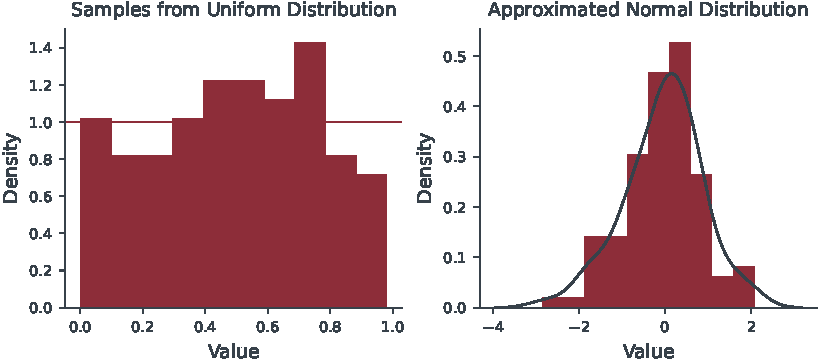
\includegraphics[scale=0.8]{../figures/inverse_cdf_normal2.pdf}
        \end{figure}
    \end{frame}
    \begin{frame}
        Number of samples = 1000:
        \begin{figure}
                \centering
                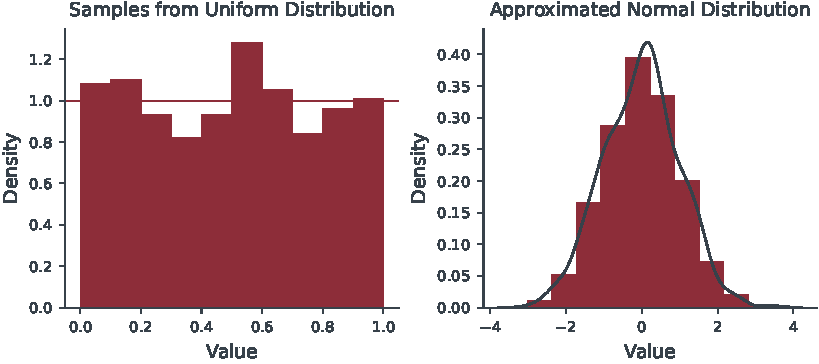
\includegraphics[scale=0.8]{../figures/inverse_cdf_normal3.pdf}
        \end{figure}
        We see that as the number of samples increases, we are able to approximate the induced distribution which is the normal distribution for this example.
    \end{frame}

    \begin{frame}{Limitations:}
        \begin{itemize}
            \item Limited Distribution Complexity: It relies on having an analytically calculable cumulative distribution function (CDF) and an invertible CDF function. 
            \item Numerical Inversion Challenges: When the inverse of the CDF cannot be expressed analytically, numerical methods introduce numerical errors and slow down the sampling process.
            \item Efficiency and Multivariate Distributions: It can be resource-intensive for high-dimensional multivariate distributions. 
        \end{itemize}
    \end{frame}
\end{section}

\begin{section}{Importance Sampling}
    \begin{frame}{General Form}
        In rejection sampling, we saw that due to less acceptance probability, a lot of samples were wasted leading to more time and higher complexity to approximate a distribution.

        Computing $p(x), q(x)$ thus seems wasteful. Let us rewrite the equation as:
        \begin{align*}
            \phi &= \int f(x)p(x)dx = \int f(x)\frac{p(x)}{q(x)}q(x)dx \\
            &\sim \frac{1}{N} \sum_{i=1}^Nf(x_i)\frac{p(x_i)}{q(x_i)} = \frac{1}{N} \sum_{i=1}^Nf(x_i)w_i 
        \end{align*}
        Here, $x_i\sim q(x)$. $w_i$ is known as the importance(weight) of sample i. 
    \end{frame}

    \begin{frame}
        However the normalization constant $Z$ is generally not known to us. Thus writing: 
        \begin{equation}
            p(x) = \frac{\Tilde{p}(x)}{Z}
        \end{equation}
        Now inserting this in earlier equations, we get:
        \begin{align*}
            \phi &=\frac{1}{Z} \int f(x)\Tilde{p}(x)dx = \frac{1}{Z}\int f(x)\frac{\Tilde{p}(x)}{q(x)}q(x)dx \\
            &\sim \frac{1}{NZ} \sum_{i=1}^Nf(x_i)\frac{\Tilde{p}(x_i)}{q(x_i)} = \frac{1}{NZ} \sum_{i=1}^Nf(x_i)w_i 
        \end{align*}
        We know that:
        \begin{align*}
            Z &= \int_{\infty}^{\infty} \Tilde{p}(x)dx = \int_{\infty}^{\infty}\frac{\Tilde{p}(x)}{q(x)}q(x)dx \\
            &= \frac{1}{N}\sum_{i=1}^N w_i
        \end{align*}
    \end{frame}

    \begin{frame}
        Substuting this value of $Z$ in the equation above, we get:
        \begin{align*}
            \phi &= \frac{1}{N}\sum_{i=1}^N f(x_i)w_i = \frac{\sum_{i=1}^N f(x_i)w_i}{\sum_{i=1}^N w_i} \\
            &= \sum_{i=1}^N f(x_i)W_i
        \end{align*}
        Here $W_i = \frac{w_i}{\sum_{i=1}^N w_i}$ are the normalized weights.
    \end{frame}

    \begin{frame}{Limitations}
        \begin{itemize}
            \item Recall that Var $\hat{\phi} = \frac{var(f)}{N}$. Importance sampling replaces $var(f)$ with $var(f\frac{p}{q})$. At positions where $p>>>q$, the weight can tend to $\infty$!
        \end{itemize}
        \begin{figure}
                \centering
                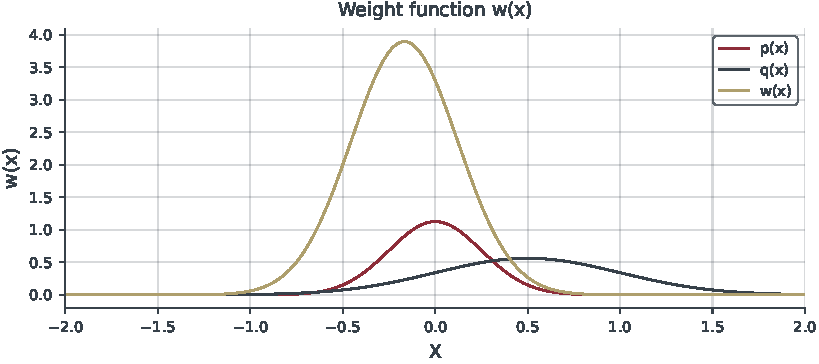
\includegraphics[scale=0.8]{../figures/importance_sampling_weight_function.pdf}
        \end{figure}
    \end{frame}
\end{section}

\begin{section}{Gibbs Sampling}
    \begin{frame}{General Form}
        Suppose we wish to sample $\theta_1, \theta_2 \sim p(\theta_1, \theta_2)$, but cannot use:\\
        \begin{itemize}
            \item direct simulation
            \item accept-reject method
            \item Metropolis-Hasting
        \end{itemize}
        But we can sample using the conditionals i.e.:\\
        \begin{itemize}
            \item $p(\theta_1|\theta_2)$ and
            \item $p(\theta_2|\theta_1)$,
        \end{itemize}
        then we can use Gibbs sampling.
    \end{frame}
    
    \begin{frame}
        Suppose $\theta_1, \theta_2 \sim p(\theta_1, \theta_2)$ and we can sample from $p(\theta_1, \theta_2)$. We begin with an initial value $(\theta_1^{0}, \theta_2^{0})$, the workflow for Gibbs algorithm is:\\
        1. sample $\theta_1^j \sim p(\theta_1|\theta_2^{j-1})$ and then\\
        2. sample $\theta_2^j \sim p(\theta_2|\theta_1^j)$.\\
        One thing to note here is that the sequence in which the theta's are sampled are not independent!    
    \end{frame}

    \begin{frame}{Bivariate Normal Example}
        Suppose \\
        $\theta \sim N_2(0,\Sigma)$ and $\Sigma = $
        $ \begin{matrix}
        1 & \rho \\
        \rho & 1  
        \end{matrix} $
    
    Then, we have:\\
    $\theta_1|\theta_2 \sim N(\rho\theta_2,[1-\rho^2])$

    $\theta_2|\theta_1 \sim N(\rho\theta_1,[1-\rho^2])$
    are the conditional distributions.
    The Gibbs sampling proceeds as follows:\\
    \begin{table}[]
        \centering
        \begin{tabular}{c c c}
           Iteration & Sample $\theta_1$ & Sample $\theta_2$\\
           \hline
           1  &  $\theta_1\sim N(\rho\theta_2^0, [1-\rho^2])$ &  $\theta_2\sim N(\rho\theta_1^1, [1-\rho^2])$\\
           & . & \\
           & . & \\
           $k$  &  $\theta_1\sim N(\rho\theta_2^{k-1}, [1-\rho^2])$ &  $\theta_2\sim N(\rho\theta_1^k, [1-\rho^2])$
             
        \end{tabular}
    \end{table}
    \end{frame}

    \begin{frame}
        \begin{figure}
                \centering
                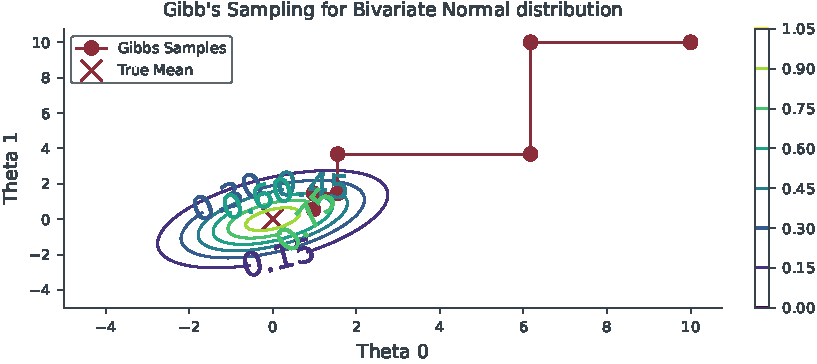
\includegraphics[scale=0.8]{../figures/gibbs_sampling_bivariate_normal.pdf}
            \end{figure}
    \end{frame}

    \begin{frame}{Multivariate case}
        Suppose $\theta = (\theta_1, \theta_2, \ldots, \theta_K)$, the Gibbs workflow is as follows:\\
        $\theta_1^j = p(\theta_1|\theta_2^{j-1}, \ldots, \theta_K^{j-1})$\\
        $\theta_2^j = p(\theta_2|\theta_1^{j}, \theta_3^{j-1}, \ldots, \theta_K^{j-1})$\\
        .\\
        .\\
        $\theta_k^j = p(\theta_k|\theta_1^{j}, \ldots, \theta_{k-1}^j, \theta_{k+1}^{j-1}, \ldots, \theta_K^{j-1})$\\
        .\\
        .\\
        $\theta_K^j = p(\theta_K|\theta_1^{j}, \ldots, \theta_{K-1}^{j})$\\
        The distributions above are call the full conditional distributions.
    \end{frame}

    \begin{frame}{Advantages}
        Gibbs sampling can be used to draw samples from $p(\theta)$ when:\\
        \begin{itemize}
            \item Other methods don't work quite well in higher dimensions.
            \item Draw samples from the full conditional distributions is easy, $p(\theta_k|\theta_{-k}).$
        \end{itemize}
    \end{frame}
\end{section}

\begin{section}{Markov Chain Monte Carlo}
    \begin{frame}{Limitations of basic sampling methods}
        \begin{itemize}
            \item \textit{Transformation based methods}: Usually limited to drawing from standard distributions.
            \item \textit{Rejection and Importance sampling}: Require selection of good proposal distirbutions.
        \end{itemize}
        In high dimensions, usually most of the density $p(x)$ is concentrated within a tiny subspace of $x$. Moreover, those subspaces are difficult to be known a priori.

        A solution to these are MCMC methods.
    \end{frame}

    \begin{frame}{Markov Chain}
        \begin{itemize}
            \item \textbf{Markov Chain}: A joint distribution $p(X)$ over a sequence of random variables $X = \{X_1, X_2, \ldots, X_n\}$ is said to have the Markov property if 
            $$
            p(X_i|X_1, \ldots, X_{i-1}) = p(X_i|X_{i-1}) 
            $$
            The sequence is then called a Markov chain.
            \item The idea is that the estimates contain information about the shape of the target distribution $p$.
        \end{itemize}
    \end{frame}

    \begin{frame}{Metropolis Hastings}
        \begin{itemize}
            \item The basic idea is propose to move to a new state $x_{i+1}$ from the current state $x_i$ with probability $q(x_{i+1}|x_i)$, where $q$ is called the proposal distribution and our target density of interest is $p (= \frac{1}{Z} \tilde{p})$.
            \item The new state is accepted with probability $\alpha(x_i, x_{i+1})$.
            \begin{itemize}
                \item If $p(x_{i+1}| x_i) = p(x_i| x_{i+1})$, then $\alpha(x_i, x_{i+1}) = \min (1, \frac{p(x_{i+1})}{p(x_i)})$.
                \item If $p(x_{i+1}| x_i) \neq p(x_i| x_{i+1})$, then $\alpha(x_i, x_{i+1}) = \min (1, \frac{p(x_{i+1})q(x_i|x_{i+1})}{p(x_i)q(x_{i+1}|x_i)}) = \min (1, \frac{\tilde{p}(x_{i+1})q(x_i|x_{i+1})}{\tilde{p}(x_i)q(x_{i+1}|x_i)})$
            \end{itemize}
            \item Evaluating $\alpha$, we only need to know the target distribution up to a constant of proportionality or without normalization constant.
        \end{itemize}
    \end{frame}

    \begin{frame}{Algorithm: Metropolis Hastings}
        \begin{enumerate}
            \item Initialize $x_0$.
            \item for $i = 1, \ldots, N$ do:
            \item \quad Sample $x^* \sim q(x^*|x_{i-1})$.
            \item \quad Compute $\alpha = \min (1, \frac{\tilde{p}(x^*)q(x_{i-1}|x^*)}{\tilde{p}(x_{i-1})q(x^*|x_{i-1})})$
            \item \quad Sample $u \sim \mathcal{U}(0, 1)$
            \item \quad if $u \leq \alpha$:
            
            \quad \quad $x_i = x^*$
            
            \quad else:
            
            \quad \quad $x_i = x_{i-1}$
        \end{enumerate}
    \end{frame}

    \begin{frame}{Pop Quiz}
        How do we choose the initial state $x_0$?
        \pause
        \begin{enumerate}
            \item Start the Markov Chain at an initial $x_0$.
            \item Using the proposal $q(x|x_i)$, run the chain long enough, say $N_1$ steps.
            \item Discard the first $N_1 - 1$ samples (called 'burn-in' samples).
            \item Treat $x_{N_1}$ as first sample from $p(x)$.
        \end{enumerate}
    \end{frame}

    \begin{frame}{MCMC demo}
        
        \url{https://chi-feng.github.io/mcmc-demo/app.html}
    \end{frame}
\end{section}

\end{document}